% !TeX root = main.tex

\hypertarget{continuity}{%
\section{Continuity}\label{continuity}}

\hypertarget{continuous-at-a-point}{%
\subsection{Continuous at a point}\label{continuous-at-a-point}}

\begin{definition}

A function \(f(x)\) is continuous at a point \(a\) if and only if the
following three conditions are satisfied:

\begin{enumerate}[sepno]
\item
  \(f(a)\) is defined
\item
  \(\lim\limits_{x\to a}f(x)\) exists
\item
  \(\lim\limits_{x\to a}f(x)=f(a)\)
\end{enumerate}

A function is discontinuous at a point \(a\) if it fails to be
continuous at \(a\).

\end{definition}

\begin{example}
Using the definition,
determine whether the function \(f(x)=\dfrac{x^2-4}{x-2}\) is continuous
at \(x=2\). Justify the conclusion.

\end{example}
\vspace*{6\baselineskip}

\begin{example}

Determining Continuity at a Point, Condition 2 Using the definition,
determine whether the function
\(f(x)=\begin{cases}-x^2+4, & \mathrm{if} \; x\le 3 \\ 4x-8, & \mathrm{if} \; x>3\end{cases}\)
is continuous at \(x=3\). Justify the conclusion.

\end{example}
\vspace*{6\baselineskip}

\begin{example}

Determining Continuity at a Point, Condition 3**\\
Using the definition, determine whether the function
\(f(x)=\begin{cases}\frac{\sin x}{x}, & \text{if } x\ne 0\\1, & \text{if } x=0\end{cases}\)
is continuous at \(x=0\).

\end{example}
\vspace*{6\baselineskip}

\hypertarget{discontinuities}{%
\subsection{Discontinuities}\label{discontinuities}}

\begin{definition}

If \(f(x)\) is discontinuous at \(a\), then

\begin{enumerate}[sepno]
\item
  \(f\) has a removable discontinuity at \(a\) if
  \(\lim\limits_{x\to a}f(x)\) exists. (Note: When we state that
  \(\lim\limits_{x\to a}f(x)\) exists, we mean that
  \(\lim\limits_{x\to a}f(x)=L\), where L is a real number.)
\item
  \(f\) has a jump discontinuity at \(a\) if
  \(\lim\limits_{x\to a^-}f(x)\) and \(\lim\limits_{x\to a^+}f(x)\) both
  exist, but
  \(\lim\limits_{x\to a^-}f(x)\neq \lim\limits_{x\to a^+}f(x)\). (Note:
  When we state that \(\lim\limits_{x\to a^-}f(x)\) and
  \(\lim\limits_{x\to a^+}f(x)\) both exist, we mean that both are
  real-valued and that neither take on the values \(\pm\infty\).)
\item
  \(f\) has an infinite discontinuity at \(a\) if
  \(\lim\limits_{x\to a^-}f(x)=\pm\infty\) or
  \(\lim\limits_{x\to a^+}f(x)=\pm\infty\).
\end{enumerate}

\end{definition}

\begin{fullwidth}
  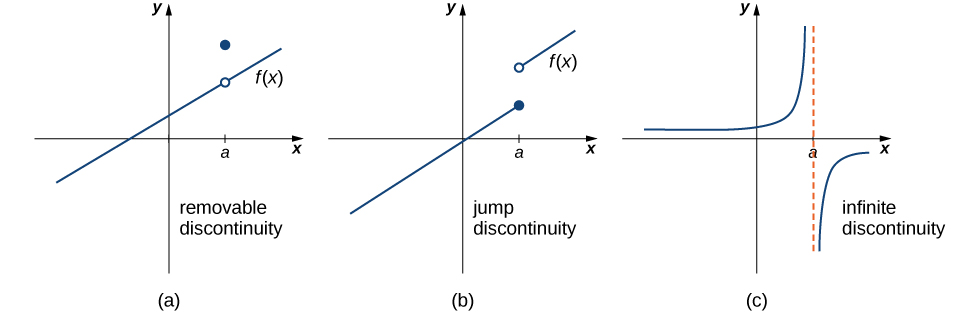
\includegraphics[width=1.2\textwidth]{img/2020-09-02-22-17-09.png}
\end{fullwidth}

\begin{example}

In Example, we showed that \(f(x)=\dfrac{x^2-4}{x-2}\) is discontinuous
at \(x=2\). Classify this discontinuity as removable, jump, or infinite.

\end{example}
\vspace*{6\baselineskip}

\hypertarget{continuity-from-the-right-and-from-the-left}{%
\subsection{Continuity from the right and from the
left}\label{continuity-from-the-right-and-from-the-left}}

\begin{definition}

  A function \(f(x)\) is said to be continuous from the right at a if
  \(\lim\limits_{x\to a^+}f(x)=f(a)\).
  
  A function \(f(x)\) is said to be continuous from the left at a if
  \(\lim\limits_{x\to a^-}f(x)=f(a)\)

\end{definition}

\hypertarget{continuity-over-an-interval}{%
\subsection{Continuity over an
interval}\label{continuity-over-an-interval}}

\begin{definition}

A function is continuous over an open interval if it is continuous at
every point in the interval. A function \(f(x)\) is continuous over a
closed interval of the form \([a,b]\) if it is continuous at every point
in \((a,b)\) and is continuous from the right at a and is continuous
from the left at b. Analogously, a function \(f(x)\) is continuous over
an interval of the form \((a,b]\) if it is continuous over \((a,b)\) and
is continuous from the left at b. Continuity over other types of
intervals are defined in a similar fashion.

\end{definition}

\begin{theorem}[Rules of continuity]

  Let \(f\) and \(g\) be two
functions continuous over an interval \(I\). Then

\begin{enumerate}[sepno]
\item
  the linear combination \(af+bg\) is continuous over the interval
  \(I\);
\item
  the multiplication \(f\cdot g\) is continuous over the interval \(I\);
\item
  the quotient \(\dfrac{f}{g}\) is continuous over the intersection of
  \(I\) and domain of \(g\).
\end{enumerate}
\end{theorem}

\begin{corollary}

Polynomials and rational functions are continuous over their domains.

\end{corollary}


\begin{example}

State the interval(s) over which the function
\(f(x)=\dfrac{x-1}{x^2+2x}\) is continuous.

\end{example}
\vspace*{6\baselineskip}

\begin{example}

State the interval(s) over which the function \(f(x)=\sqrt{4-x^2}\) is
continuous.

\end{example}
\vspace*{6\baselineskip}

\hypertarget{continuity-of-composite-functions}{%
\subsection{Continuity of Composite
Functions}\label{continuity-of-composite-functions}}

\begin{theorem}

If \(f(x)\) is continuous at \(L\) and \(\lim\limits_{x\to a}g(x)=L\),
then
\(\lim\limits_{x\to a}f\big(g(x)\big)=f\big(\lim\limits_{x\to a}g(x)\big)=f(L).\)
In particular, if \(g\) is continuous at \(a\), then \(f\circ g\) is
continuous at \(a\).

\end{theorem}

\begin{example}

Evaluate the limit \(\lim\limits_{x\to 0}\frac{\sin^2x}{x^2}.\)

\end{example}
\vspace*{6\baselineskip}

\hypertarget{continuity-of-trigonometric-functions}{%
\subsection{Continuity of Trigonometric
Functions}\label{continuity-of-trigonometric-functions}}

\begin{theorem}

Trigonometric functions are continuous over their entire domains.

\end{theorem}

% \textbf{Sketch of proof:}

% \begin{enumerate}
% \item
%   Since \(-x<\sin x<x\), by squeeze theorem, we know \(\sin x\) is
%   continuous at \(x=0\).
% \item
%   By the sum angle formula
%   \(\cos x=\cos(x-\frac\pi2+\pi)=\cos(x-\frac\pi2)\cos(\frac\pi2)-\sin(x-\frac\pi2)\sin(\frac\pi2)\).
%   Apply the theorem of continuity of composite functions to
%   \(\sin(x-\frac\pi2)\), we know that \(\lim\limits_{x\to 0}\cos x=1\).
% \item
%   By the theorem of continuity of composite function again, we see that
%   \(\lim\limits_{x\to a}\sin(x-a)=0\) and
%   \(\lim\limits_{x\to a}\cos(x-a)=1\) for any real number \(a\).
% \item
%   For any real number \(a\), the limit \(\lim\limits_{x\to a}\sin x\)
%   can be calculate using the formula of sum of two angles
%   \[\sin((x-a)+a)=\sin(x-a)\cos a+\cos(x-a)\sin a.\]
% \end{enumerate}

\begin{example}

Evaluate the limit \(\lim\limits_{x\to 0}\cos(3x)\).

\end{example}
\vspace*{6\baselineskip}

\hypertarget{the-intermediate-value-theorem}{%
\subsection{The Intermediate Value
Theorem}\label{the-intermediate-value-theorem}}

\begin{theorem}[Intermediate Value Theorem]

  Let \(f\) be continuous over a closed, bounded interval \([a,b]\). If \(z\) is any real number between \(f(a)\)
and \(f(b)\), then there is a number c in \([a,b]\) satisfying
\(f(c)=z\).

\end{theorem}

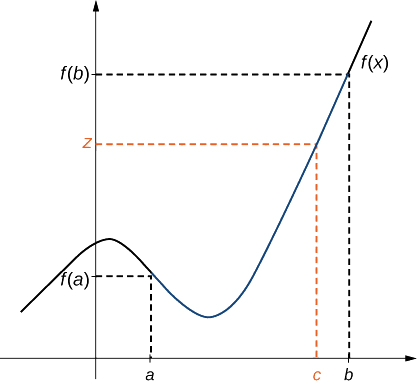
\includegraphics{img/2.4.3.png}

\begin{example}

Show that \(f(x)=x-\cos x\) has at least one zero.

\end{example}
\vspace*{6\baselineskip}

\subsection{Practice}





\begin{exercise}

  Using the definition, determine whether the function
  \(f(x)=\begin{cases}2x+1, & \text{if }x<1\\2, & \text{if }x=1\\ -x+4, & \text{if }x>1\end{cases}\)
  is continuous at \(x=1\). If the function is not continuous at 1,
  indicate the condition for continuity at a point that fails to hold.
  
  \end{exercise}
  \vspace*{6\baselineskip}
  
\begin{exercise}

Classify this discontinuity as removable, jump, or infinite.

\begin{enumerate}
\item
  Determine whether \(f(x)=\dfrac{x+2}{x+1}\) is continuous at \(-1\).
  If the function is discontinuous at \(-1\), classify the discontinuity
  as removable, jump, or infinite.
\item
  Determine whether
  \(f(x)=\begin{cases}x^2, &\text{if }x\ne 1\\3, & \text{if }x=1\end{cases}\)
  is continuous at \(1\). If \(f\) is not continuous at \(1\), classify
  the discontinuity as removable, jump, or infinite.
\item
  Determine whether the function
  \(f(x)=\begin{cases}-x+1, & \mathrm{if} \; x\le 2 \\ x^2-3, & \mathrm{if} \; x>2\end{cases}\)
  is continuous at \(x=2\). If \(f\) is not continuous at \(1\),
  classify the discontinuity as removable, jump, or infinite.
\end{enumerate}

\end{exercise}

\begin{exercise}

State the interval(s) over which the function
\(f(x)=\frac{x-1}{\sqrt{x+3}}\) is continuous.

\end{exercise}
\vspace*{6\baselineskip}

\begin{exercise}

Evaluate the limit \(\lim\limits_{x\to \frac\pi3}\tan(2\pi-3x)\).

\end{exercise}
\vspace*{6\baselineskip}

\begin{exercise}

Show that \(f(x)=x^3-x^2-3x+1\) has a zero over the interval \([0,1]\).

\end{exercise}
\vspace*{6\baselineskip}

\begin{exercise}

For \(f(x)=1/x,f(-1)=-1<0\) and \(f(1)=1>0\). Can we conclude that
\(f(x)\) has a zero in the interval \([-1,1]\)?

\end{exercise}
